\section{Introduction}

Complex cyber-physical systems (\ie, advanced embedded real-time computing systems) have \emph{timeliness} requirements %over computation 
such that associated deadlines must be met (\eg, for safety-critical systems). Appropriate analytical techniques have been developed that enable \emph{a priori} guarantees to be established over timing behaviour at run-time regarding computation deadlines.  
The seminal work by Liu and Layland \cite{Liu_1973} considers the scheduling of periodic computation (termed \emph{tasks}). 
Analysis presented enables the \emph{schedulability} of a set of such tasks to be established, \ie, whether their deadlines will be met at run-time. This has been extended to incorporate many other task characteristics, \eg, sporadic tasks\cite{Mok:1983:FDP:888951}. 

One underlying assumption of the majority of these schedulability analyses is that a task does not voluntarily suspend its execution -- once executing, a task can only stop as a result of preemption by a higher priority task, becoming blocked on a shared resource that is held by another lower-priority job on the same processor, or completing its execution for that release of the task (\ie, meeting its deadline). The alternative, that a task can \emph{self-suspend}, means that the assumptions underpinning basic analysis no longer hold. As an example, consider the execution scenario in Figure~\ref{fig:ss-intuition}. In Figure \ref{fig:ss-intuition}(a) the classical worst case is illustrated, where the longest time that a task will execute before completing its execution occurs at a release coinciding with the release of all higher priority tasks (termed \emph{critical instant}). As Figure \ref{fig:ss-intuition}(b) shows, when a higher-priority task  has suspended its execution time, the result is that the lower-priority task now misses its deadline.


Self-suspension has become increasingly important to model accurately within schedulability analysis. For example, a task that utilizes an accelerator or external physical device~\cite{Kang:rtss07,Kato_2011} where the resulting suspension delays range from a few microseconds (\eg, a write operation on a flash drive~\cite{Kang:rtss07}) to a few hundreds of milliseconds (\eg, offloading computation to GPUs~\cite{Kato_2011,Liu_2014}).  Whilst the maximum self-suspension time could be included as additional execution time, this would be pessimistic and potentially under-utilize the processor at run-time -- if the self-suspension is for a substantial time, it is advantageous to execute an alternative task.

This paper seeks to provide the first survey of existing analyses for tasks that may self-suspend, highlighting the deficiencies within these analyses. The remainder of this section provides more background and motivation of general self-suspension and the issues it causes for analysis, followed by a thorough outline of the remainder of this survey paper.


% \begin{figure}[t]
% \begin{center}
% 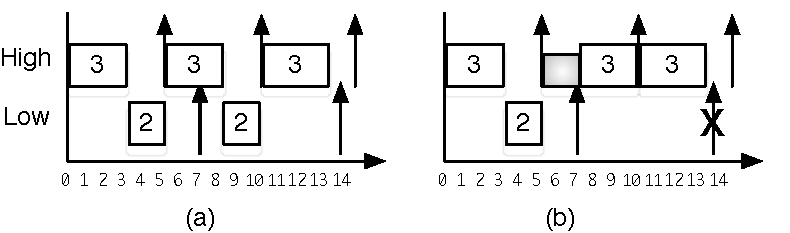
\includegraphics[width=\linewidth]{../figures/SelfSuspensionIntuition.pdf}
% \end{center}
% \caption{Two tasks \emph{High} (period 5, computation time 3) and \emph{Low} (period 7, computation time 2) meet their deadlines in (a). Conventional schdulability analysis will predict maximum response times of 3 and 5 respectively. In (b), task \emph{High} self suspends (indicated by shaded box), with the result that \emph{Low} will miss its deadline at time 14.}
% \label{fig:ss-intuition}
% \end{figure}


\begin{figure}[t]
\centering
\def\uxfpga{0.4cm} 
\subfloat[]{\scalebox{0.76}{
	\begin{tikzpicture}[x=\uxfpga,y=\uy,auto, thick]
    \draw[->] (0,0) -- coordinate (xaxis) (16,0) node[anchor=north]{$t$};
    \draw[] (0,2) -- coordinate (xaxis) (16,2) node[anchor=north]{};
    \foreach \x in {0,1,...,15}{
      \draw[-,below](\x,0) -- (\x,-0.3) node[] {\pgfmathtruncatemacro\yi{\x} \yi};
    }
    \foreach \x in {0,5,10,15}{
      \draw[-,very thin,lightgray, dashed](\x,0.3) -- (\x,4);
    }	
    
    \begin{scope}[shift={(0,0)}]
      \node[anchor=east] at (0, 0.5) {$\tau_2 (low)$};
    \foreach \x in {0,7,14}{ 
        \draw[->] (\x,0) -- (\x,1.75);        		
      }
      \foreach \x in {3,8}{ 
        \node[task7, minimum width=2*\uxfpga, anchor=south west] at (\x, 0){};
      }
    \end{scope}
    
    \begin{scope}[shift={(0,2)}]
      \node[anchor=east] at (0, 0.5) {$\tau_1 (high)$};
      \foreach \x in {0,5,10,15}{ 
        \draw[->] (\x,0) -- (\x,1.75);        		
      }
      \foreach \x in {0,5,10}{ 
        \node[task7, minimum width=3*\uxfpga, anchor=south west] at (\x, 0){};
      }
    \end{scope}                
  \end{tikzpicture}}}
\subfloat[]{\scalebox{0.76}{
	\begin{tikzpicture}[x=\uxfpga,y=\uy,auto, thick]
    \draw[->] (0,0) -- coordinate (xaxis) (16,0) node[anchor=north]{$t$};
    \draw[] (0,2) -- coordinate (xaxis) (16,2) node[anchor=north]{};
    \foreach \x in {0,1,...,15}{
      \draw[-,below](\x,0) -- (\x,-0.3) node[] {\pgfmathtruncatemacro\yi{\x} \yi};
    }
    \foreach \x in {0,5,10,15}{
      \draw[-,very thin,lightgray, dashed](\x,0.3) -- (\x,4);
    }	
    
    \begin{scope}[shift={(0,0)}]
      \node[anchor=east] at (0, 0.5) {$\tau_2 (low)$};
    \foreach \x in {0,7,14}{ 
        \draw[->] (\x,0) -- (\x,1.75);        		
      }
      \foreach \x in {3,13}{ 
        \node[task7, minimum width=2*\uxfpga, anchor=south west] at (\x, 0){};
      }
      \draw[very thick, red](13.5, 0.3) -- (14.5, 1);
      \draw[very thick, red](13.5, 1) -- (14.5, 0.3);
    \end{scope}
    
    \begin{scope}[shift={(0,2)}]
      \node[anchor=east] at (0, 0.5) {$\tau_1 (high)$};
      \foreach \x in {0,5,10,15}{ 
        \draw[->] (\x,0) -- (\x,1.75);        		
      }
      \foreach \x in {0,7,10}{ 
        \node[task7, minimum width=3*\uxfpga, anchor=south west] at (\x, 0){};
      }
      \draw(6.2, 1.25) node{\tiny suspend};
      \draw(5, 0.3) -- ( 7,0.3);
      \draw(5, 0.5) -- ( 7,0.5);
      \draw(5, 0.7) -- ( 7,0.7);
    \end{scope}         
  \end{tikzpicture}}}
\caption{
Two tasks $\tau_1$ (higher priority, period 5, computation time 3) and $\tau_2$ (lower priority, period 7, computation time 2) meet their deadlines in (a). Conventional schdulability analysis will predict maximum response times of 3 and 5 respectively. In (b), task $\tau_1$ suspends itself, with the result that task $\tau_2$ will miss its deadline at time 14.}
\label{fig:ss-intuition}
\end{figure}


%For over half a centry, researchers in real-time systems have devoted themselves to effective design and efficient analyses of different recurrent task models to ensure that tasks can meet their specified deadlines. In most of these studies, \emph{task suspensions are usually not allowed}. That is, after a job is released, the job is either executed or stays in the ready queue, but it is not moved to the suspension state. 
 %Such an assumption is valid only under the following conditions: (1) the latency of the memory accesses and I/O peripherals is considered to be part of the worst-case execution time of a job, (2) there is no external device for accelerating the computation, and (3) there is no synchronization between different tasks on different processors in a multiprocessor or distributed computing platform.


%Due to the evolution in computer architecture towards using multicore systems and accelerators, self-suspension behaviour has become more visible in designing real-time embedded systems.  The suspension-oblivious approach, which considers the suspension time as computation, can be very pessimistic if the suspension time is long. Self-suspensions have been even more pervasive in many emerging embedded cyber-physical systems in which the computational components frequently interact with external and physical devices~\cite{Kang:rtss07,Kato_2011}.  Typically, the resulting suspension delays range from a few microseconds (\eg, a write operation on a flash drive~\cite{Kang:rtss07}) to a few hundreds of milliseconds (\eg, offloading computation to GPUs~\cite{Kato_2011,Liu_2014}). 



\subsection{Impact of Self-Suspending Behaviour}

When the self-suspending behaviour is present in the periodic/sporadic task model, the scheduling problem becomes much harder to handle. In the ordinary periodic task model, Liu and Layland showed that the earliest-deadline-first (EDF) scheduling algorithm is an optimal scheduling policy to meet all deadlines and the rate-monotonic (RM) scheduling algorithm is an optimal fixed-priority (FP) scheduling policy to meet all deadlines \cite{Liu_1973}. However, the introduction of suspension behaviour has a negative impact on the timing predictability and causes intractability in hard real-time systems~\cite{Ridouard_2004}. It was shown by Ridouard et al. \cite{Ridouard_2004} that finding an optimal schedule (to meet all deadlines) is ${\cal NP}$-hard in the strong sense even when the suspending behaviour is known a priori.


One specific problem due to self-suspending behaviour is the \emph{deferrable} execution phenomena. In the ordinary sporadic and periodic task model, the critical instant theorem by Liu and Layland \cite{Liu_1973} provides concrete worst-case scenarios for fixed-priority scheduling.  That is, the critical instant of a task defines the instant at which, considering the state of the system, an execution request for the task will generate the worst-case response time (if the job completes before next jobs of the task are released).
However, with self-suspensions, no critical instant theorem has yet been established.
% Even worse, the suspending behaviour incurs the jitter of the workload to be executed. 
Therefore, when real-time tasks may suspend, the system behaviour may become very different. For example, it is known that EDF (RM, respectively) has a $100\%$ ($69.3\%$, respectively) utilization bound for ordinary periodic real-time task systems by Liu and Layland \cite{Liu_1973}. However, with self suspensions,  it was shown in \cite{Ridouard_2004,RTSS-ChenL14} that most existing scheduling strategies, including EDF and RM, do not perform well, in the sense that they do not provide any bounded performance guarantees. 

Self-suspending tasks can be classified into two models: \emph{dynamic} self-suspension and \emph{segmented} (or \emph{multi-segment}) self-suspension models.
The dynamic self-suspension sporadic task model characterizes each
task $\tau_i$ with predefined worst-case execution time and worst-case self-suspending time, in which self-suspension can take place as long as it does not suspend longer than the specified worst case. The segmented self-suspending sporadic task model defines the execution behaviour of a job of a task by predefined computation segments and self-suspension intervals.  

\subsection{Purpose and Organization of This Paper}
There have been several research efforts, focusing on the design of scheduling algorithms and schedulability analysis of task systems when self-suspending tasks are present. Due to the prevailing self-suspending scenarios in modern computing systems, several results in the literature have been recently re-examined. We have found out that the literature of real-time scheduling for self-suspending task systems has been seriously flawed. Several misconceptions were adopted in the literature including 
\begin{itemize}
\item Incorrect quantification of jitter for dynamic self-suspending
  task systems, which was used in
  \cite{ECRTS-AudsleyB04,RTAS-AudsleyB04,RTCSA-KimCPKH95,MingLiRTCSA1994}.  This
  misconception was unfortunately adopted in \cite{zeng-2011,bbb-2013,yang-2013,kim-2014,han-2014,carminati-2014,yang-2014,lakshmanan-2009} to analyze the worst-case response time for
  partitioned multiprocessor real-time locking protocols.
\item Incorrect quantification of jitter for dynamic self-suspending
  task systems, which was used in  \cite{RTCSA-BletsasA05}.
\item Incorrect assumptions in the critical instant with
  synchronous releases, which was used in \cite{LR:rtas10}.
\item Incorrectly counting highest-priority self-suspending time to reduce
  interference, which was used in  \cite{RTSS-KimANR13}. 
\item Incorrect segmented fixed-priority scheduling with period
  enforcement, which was used in \cite{RTSS-KimANR13,DBLP:journals/ieicet/DingTT09}.
\end{itemize}


\noindent Due to the above misconceptions and the lack of a survey and review paper of this research area, the authors, who have worked in this area in the past years, have jointly worked together to review the existing results in this area. This review paper serves to
\begin{itemize}
\item summarize the existing self-suspending task models in Section~\ref{sec:model}, 
\item provide the general methodologies to handle self-suspending task systems in hard real-time systems in Section~\ref{sec:review} and soft real-time systems in Section~\ref{sec:soft-realtime}, 
\item explain the misconceptions in the literature, their consequences, and potential solutions to fix those flaws in Section~\ref{sec:misconceptions}, 
\item examine the inherited flaws in multiprocessor synchronization, due to the flawed analysis in self-suspending task models, in Section~\ref{sec:syn}, and
\item provide the summary of the computational complexity classes of different self-suspending task models and systems in Section~\ref{sec:hardness}.
\end{itemize}
Some results in the literature are listed with open issues that require further detailed examination to confirm their correctness. These are listed in Section~\ref{sec:open-issues-existing}. 
% We have also listed the potential future research topics pertaining to self-suspending task models in Section~\ref{sec:open-issues-future}.

During the preparation of this review paper, several reports, \ie, \cite{ChenHuangNelissen,ChenBrandenburg,erratu-cong-anderson,BletsasReport2015}, have been filed to discuss the flaws, the limits, and the proofs of individual papers and methods. This review paper would become too lengthy if we had to include all of them in detail.  The purpose of this review is not to present the individual discussions, evaluations and comparisons of the results in the literature. Our focus of this review is to provide a systematic picture of this research area, the misconceptions, and the state of the art of self-suspending task scheduling. Although it is unfortunate that many results in this area were flawed due to some misconceptions that are seemingly correct, we hope that this review can serve as a milestone in this research area to provide a solid base for future research to cope with self-suspending task systems.







%%% Local Variables:
%%% mode: latex
%%% TeX-master: "JRTS/JRTS.tex"
%%% End:


    
  

    
  
